% ---------------------------------------------------------------------
% ---------------------------------------------------------------------
% ---------------------------------------------------------------------

\chapter[Introduction]{Introduction}
\label{chap:intro}

Networks are fundamental in science because they provide a way to model complex systems and relationships between entities. By representing entities as nodes and connections between them as edges, networks can help researchers understand how information, energy, materials, and other resources flow through a system, identify patterns and structures within the data, and make predictions about system behavior. Many real life problems can be modeled as networks or graphs and that is why they are used in many fields, including biology, physics, sociology, and computer science, and have led to significant advances in our understanding of the world around us.

\section{Mathematical notation}
\label{sec:graph}
A network or graph in mathematical literature is, in its simplest form, a collection of interconnected nodes or vertices that represent entities, and the connections or edges between these nodes that represent relationships or interactions between the entities. Graphs are usually described using a combination of mathematical notation and visual diagrams to provide a complete representation of the network structure and properties. The \emph{adjacency matrix} of a network with $N$ nodes is defined as $\mathbf{A}\in\mathbb{R}^{N\times N}$ with elements such as:

\begin{equation}
  A_{ij} =
    \begin{cases}
      1 & \text{if there is an edge between nodes $i$ and $j$}\\
      0 & \text{otherwise}
    \end{cases}       
\end{equation}

Additionally, graphs can be represented visually using a diagram, where nodes are represented as points and edges are represented as lines connecting the points. The direction of the edges (\textit{directed} or \textit{undirected}) and the presence of loops (edges connecting a node to itself) can also be indicated in the visual representation.

Some other relevant network properties in Graph Theory that will be mentioned later in this thesis are the following:
\begin{itemize}
  \item \textit{Weighted networks}: A weighted network is a graph in which each edge has a weight or strength assigned to it. These weights represent the strength or importance of the connections between nodes. \textit{Unweighted networks} are those when no weight is assigned.
  \item \textit{Static networks}: A static network is a network that does not change over time. The relationships and connections between nodes are fixed and remain constant. 
  \item \textit{Dynamic networks}: A dynamic network is a network that changes over time. The relationships and connections between nodes can evolve and alter, resulting in a continually changing network structure.
\end{itemize}

Linear algebra will also play a significant role in network analysis as graphs can be represented as matrices. The analysis of networks often involves solving linear systems, determining eigenvalues and eigenvectors, and evaluating matrix functions. Additionally, the examination of dynamic processes on graphs will create systems of differential equations based on their structure. The behavior of the solution over time is highly impacted by that graph's structure (topology), which is reflected in the spectral properties of the matrices related to the graph. That is why one of the most basic questions about network structure is the identification of the relevant nodes in a network which leads us to the concept of centrality.

\section{Centrality measures}
\label{sec:centra}
 Centrality measures are metrics that are used to quantify the relative importance or influence of a node in a network. Indicators of centrality assign numbers or rankings, the higher the more important, to nodes within a graph corresponding to their network position based on different criteria giving rise to several types of centrality measures:

\subsection*{Degree Centrality} Measures the number of connections a node has to other nodes in the network.

\subsection*{Closeness Centrality} Measures the average distance between a node and all other nodes in the network.

\subsection*{Betweenness Centrality} Measures the number of times a node acts as a bridge along the shortest path between two other nodes in the network.

\subsection*{Eigenvector Centrality} Measures the influence of a node based on the influence of its neighbors.

\subsection*{Katz Centrality}

\subsection*{Page Rank}

Each centrality measure provides a different perspective on the importance of a node in a network and can be useful in various applications, such as social network analysis, recommendation systems, and identifying key players in complex systems.

-- when choosing Katz or PR--

\begin{figure}[htbp]\centering
	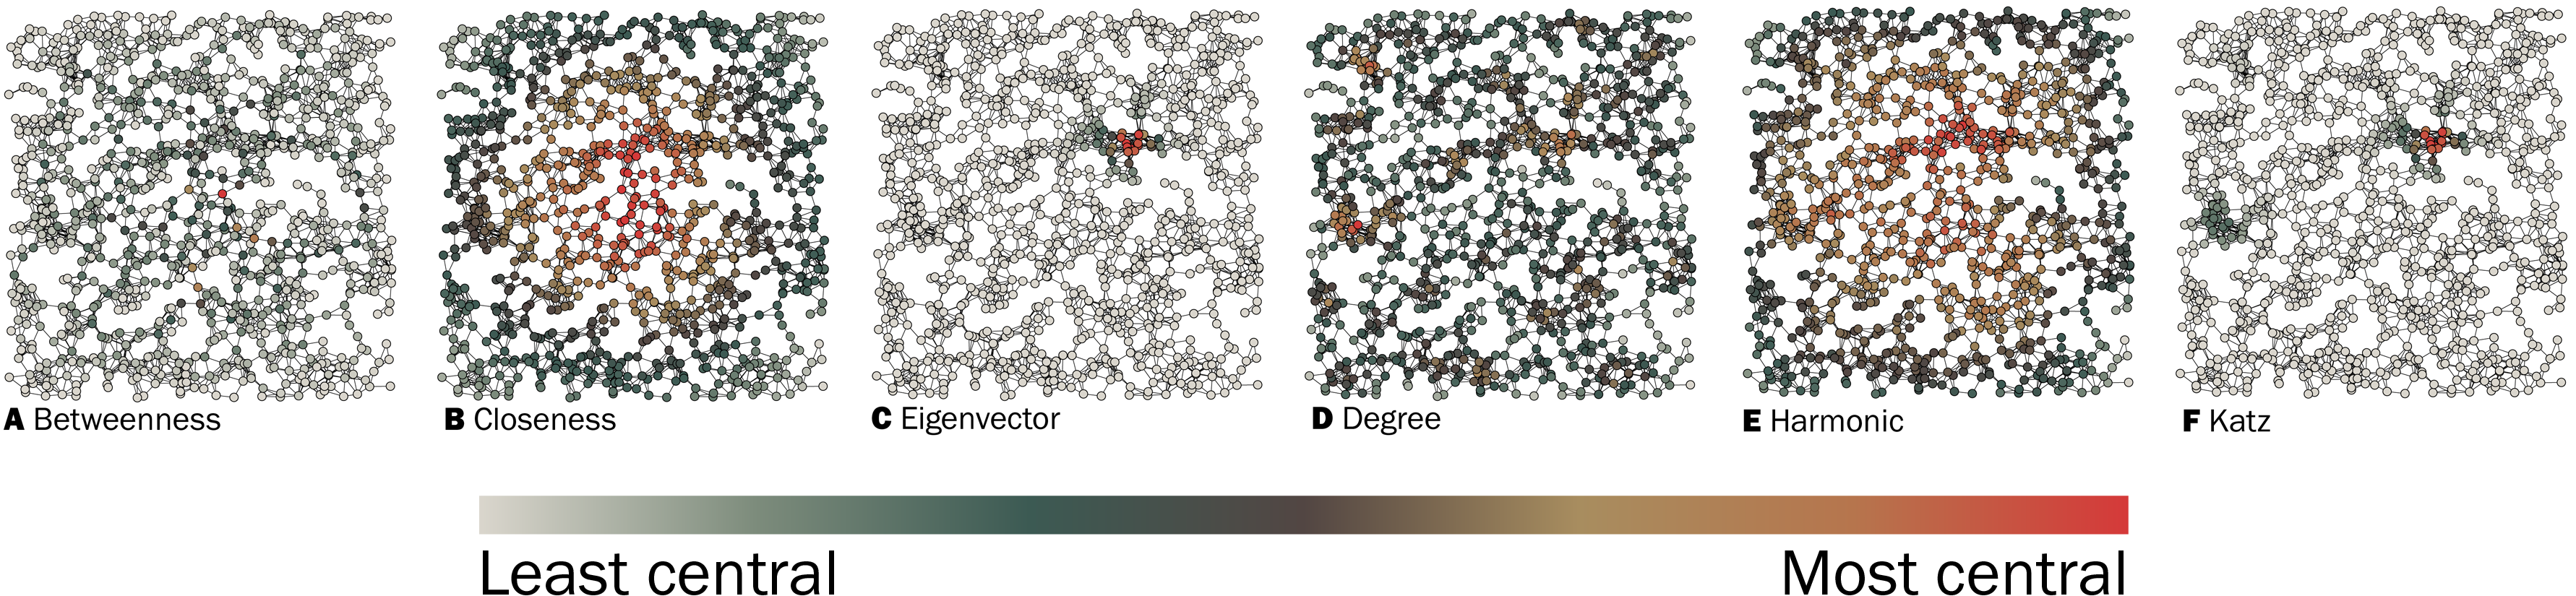
\includegraphics[width=.85\textwidth]{centrality}
	\caption{Centrality measures}
	\label{centrality}
	\bigskip
\end{figure}

\section{Background on Katz centrality in static networks}
\label{sec:back}
Text.

\section{Motivation of the study}
\label{sec:motiv}
Text.


Lacus viverra vitae congue eu consequat ac felis donec. Ultrices dui sapien eget mi proin sed libero enim. Id consectetur purus ut faucibus pulvinar elementum integer\index{Integer}. In massa tempor nec feugiat \textsl{Newman} \cite{newman2018networks}.
% ---------------------------------------------------------------------
% ---------------------------------------------------------------------
